\chapter{Introdução}

\section{Motivação}
Há uma expectativa de que, no ano de 2017, o número de casas inteligentes aumente cerca de 17\% nos Estados Unidos \cite{mckinseyReport}, onde já se tem investimentos de grandes empresas, como Google, Amazon e Apple. O interesse nessa área é tamanho que a Google investiu cerca de 5 milhões de dólares em um comercial de seu produto Google Home no Super Bowl 2017, jogo que decide o time campeão da temporada de futebol americano nos EUA \cite{kennemer}. É esperado que os consumidores invistam cada vez mais em casas inteligentes nos próximos anos, com previsões de que o valor total desse mercado chegue a mais de 63 bilhões de dólares em 2020 \cite{businessWire}.

As aplicações de automação residencial não mais se limitam a sistemas de iluminação e controle da ventilação e temperatura de cômodos. Elas contemplam também segurança, eficiência energética e até mesmo soluções voltadas à área da saúde, com dispositivos voltados especificamente a pessoas idosas, com problemas de mobilidade ou doenças crônicas \cite{iscoop}.

Os avanços das tecnologias de Internet das Coisas (\textit{Internet of Things} ou IoT) apontam para um futuro no qual qualquer dispositivo da casa possa estar conectado à Internet, criando uma série de possibilidades para a criação de integrações e funcionalidades inteligentes para o dia-a-dia. É previsto que o número de conexões \textit{Machine to Machine} (M2M) de dispositivos de casa conectada tenha uma taxa de crescimento composta de 18\% entre 2016 e 2021 \cite{ciscoReport}.

\begin{figure}[H]
	\centering
	\caption{Crescimento do número de conexões M2M por tipo de aplicação}
  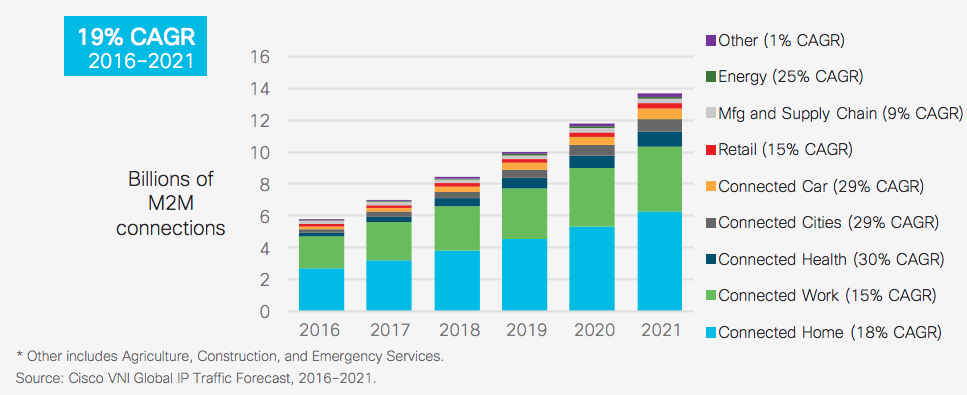
\includegraphics[width=0.2\textwidth]{m2mGrowth}
	\caption*{Fonte: \cite{ciscoReport}}
\label{fig:m2mGrowth}
\end{figure}

As oportunidades trazidas pelo conceito de IoT à área de automação residencial são uma grande motivação para esse projeto. Também destaca-se a possibilidade de promover tais tecnologias de casas inteligentes ao mercado nacional, personalizando produtos e adequando-as às necessidades dos potenciais consumidores brasileiros. Mesmo nos Estados Unidos, ainda é necessário algum tempo até que as casas conectadas se consolidem, de modo que há grandes oportunidade de pioneirismo no mercado brasileiro, com o lançamento de produtos de IoT a preços acessíveis e focando nas necessidades dos consumidores locais.

\section{Projeto Hedwig}

\subsection{Objetivo}
A contribuição do projeto será um sistema baseado em arquitetura local modularizada, e em camadas, com funcionalidades local e em nuvem, e provedor de uma \textit{API} que permita seu acesso por diversos clientes - como \textit{websites} ou aplicativos para \textit{smartphones} - que seja capaz de monitorar e agir em diversos módulos presentes na residência do usuário final do sistema. O projeto irá disponibilizar módulos físicos, prontos para serem instalados e configurados na residência, sem que seja necessário conhecimentos avançados de eletrônica ou computação.

Desta forma, os principais pontos do projeto são:

\begin{description}
\item \textbf{Robustez}

3 níveis de funcionamento: Online, Local e Offline, para garantir a disponibilidade mesmo com problemas (queda do servidor, internet indisponível, falha no roteador), com medidas para a tentativa automática de reconexão, monitoramento e manutenções preventivas e corretivas do sistema.

\item \textbf{Modularidade}

Garante a independência de funcionamento dos módulos que atendem às várias necessidades, contribuindo para a robustez. Diminui o custo e personaliza o produto, de acordo com as necessidades do cliente.

\item \textbf{Camadas}

O funcionamento da aplicação decorre em diversos níveis e camadas, de responsabilidades independentes, permitindo maior separação de responsabilidades.

\item \textbf{Machine Learning}

Geração de aprendizado de máquina por meio de análise automática do uso do sistema pelos usuários, de forma a analisar suas rotinas e poder atuar em cima de tais informações por meio de notificações, alertas e acionamentos automáticos de funções para o usuário.

\item \textbf{Segurança}

Utilização de criptografia assimétrica para comunicação entre servidor local e serviços de nuvem, juntamente com conexão por \textit{WebSocket}. Autenticação e autorização de usuários com utilização de \textit{JSON Web Tokens}. Uso de canais \textit{Publisher/Subscriber} protegidos para troca de mensagens.

\end{description}

\subsection{Nome do Projeto}
O nome do projeto foi escolhido em homenagem a Hedy Lamarr. Nascida Hedwig Eva Maria Kiesler \cite{shearer}, a atriz e inventora desenvolveu, durante a Segunda Guerra Mundial, um aparelho de interferência em rádio para despistar radares nazistas, cujos princípios estão incorporados nas tecnologias atuais de Wi-Fi, CDMA e Bluetooth \cite{electronicFrontier}. Baseado na ideia de um sistema de comunicação seguro, e como reconhecimento de seu trabalho, foi dado esse nome ao projeto aqui descrito.

\subsection{Logo}
O logo do projeto é uma coruja, em referência à coruja \textit{Hedwig} do personagem \textit{Harry Potter}, da série de livros de mesmo nome.
\begin{figure}[H]
	\centering
	\caption{Projeto Hedwig}
  
\includegraphics[width=0.2\textwidth]{hedwigLogo}
\label{fig:hedwigLogo}
\end{figure}

\section{Aplicações}
Como aplicações do projeto Hedwig, destacam-se a automação no uso de eletrodomésticos e iluminação, segurança no acesso à casa, economia nas contas de água e energia elétrica, além de um monitoramento remoto de pessoas que moram sozinhas (como é o caso de idosos), garantindo a tranquilidade de seus familiares e mantendo a segurança do indivíduo.

Exemplos de módulos que podem ser incluídos no sistema são: quarto (despertador, iluminação, monitoramento de temperatura e umidade); cozinha (\textit{timer}, iluminação, monitoramento de presença e gás); acesso (controle de abertura, monitoramento de estado); externo (monitoramento de temperatura, umidade, energia elétrica e consumo de água); corredor (monitoramento de presença, iluminação), chuveiro (controle de temperatura\slash potência a partir do perfil de usuário e temperatura externa) e ar condicionado (controle da potência a partir do monitoramento das temperaturas internas e externas da casa).

A presença de funcionalidades de Machine Learning incrementa o sistema, permitindo trazer facilidades aos usuários. O sistema torna-se capaz de aprender com os feedbacks do usuário, seja pelo monitoramento dos módulos ou por respostas dadas por meio do aplicativo, e pode atuar em questões de segurança (\textit{safety}), saúde e automação da residência do cliente.
